\documentclass[]{book}
\usepackage{lmodern}
\usepackage{amssymb,amsmath}
\usepackage{ifxetex,ifluatex}
\usepackage{fixltx2e} % provides \textsubscript
\ifnum 0\ifxetex 1\fi\ifluatex 1\fi=0 % if pdftex
  \usepackage[T1]{fontenc}
  \usepackage[utf8]{inputenc}
\else % if luatex or xelatex
  \ifxetex
    \usepackage{mathspec}
  \else
    \usepackage{fontspec}
  \fi
  \defaultfontfeatures{Ligatures=TeX,Scale=MatchLowercase}
\fi
% use upquote if available, for straight quotes in verbatim environments
\IfFileExists{upquote.sty}{\usepackage{upquote}}{}
% use microtype if available
\IfFileExists{microtype.sty}{%
\usepackage{microtype}
\UseMicrotypeSet[protrusion]{basicmath} % disable protrusion for tt fonts
}{}
\usepackage{hyperref}
\hypersetup{unicode=true,
            pdftitle={Introduction to HTA in R},
            pdfauthor={Nathan Green},
            pdfborder={0 0 0},
            breaklinks=true}
\urlstyle{same}  % don't use monospace font for urls
\usepackage{natbib}
\bibliographystyle{apalike}
\usepackage{color}
\usepackage{fancyvrb}
\newcommand{\VerbBar}{|}
\newcommand{\VERB}{\Verb[commandchars=\\\{\}]}
\DefineVerbatimEnvironment{Highlighting}{Verbatim}{commandchars=\\\{\}}
% Add ',fontsize=\small' for more characters per line
\usepackage{framed}
\definecolor{shadecolor}{RGB}{248,248,248}
\newenvironment{Shaded}{\begin{snugshade}}{\end{snugshade}}
\newcommand{\AlertTok}[1]{\textcolor[rgb]{0.94,0.16,0.16}{#1}}
\newcommand{\AnnotationTok}[1]{\textcolor[rgb]{0.56,0.35,0.01}{\textbf{\textit{#1}}}}
\newcommand{\AttributeTok}[1]{\textcolor[rgb]{0.77,0.63,0.00}{#1}}
\newcommand{\BaseNTok}[1]{\textcolor[rgb]{0.00,0.00,0.81}{#1}}
\newcommand{\BuiltInTok}[1]{#1}
\newcommand{\CharTok}[1]{\textcolor[rgb]{0.31,0.60,0.02}{#1}}
\newcommand{\CommentTok}[1]{\textcolor[rgb]{0.56,0.35,0.01}{\textit{#1}}}
\newcommand{\CommentVarTok}[1]{\textcolor[rgb]{0.56,0.35,0.01}{\textbf{\textit{#1}}}}
\newcommand{\ConstantTok}[1]{\textcolor[rgb]{0.00,0.00,0.00}{#1}}
\newcommand{\ControlFlowTok}[1]{\textcolor[rgb]{0.13,0.29,0.53}{\textbf{#1}}}
\newcommand{\DataTypeTok}[1]{\textcolor[rgb]{0.13,0.29,0.53}{#1}}
\newcommand{\DecValTok}[1]{\textcolor[rgb]{0.00,0.00,0.81}{#1}}
\newcommand{\DocumentationTok}[1]{\textcolor[rgb]{0.56,0.35,0.01}{\textbf{\textit{#1}}}}
\newcommand{\ErrorTok}[1]{\textcolor[rgb]{0.64,0.00,0.00}{\textbf{#1}}}
\newcommand{\ExtensionTok}[1]{#1}
\newcommand{\FloatTok}[1]{\textcolor[rgb]{0.00,0.00,0.81}{#1}}
\newcommand{\FunctionTok}[1]{\textcolor[rgb]{0.00,0.00,0.00}{#1}}
\newcommand{\ImportTok}[1]{#1}
\newcommand{\InformationTok}[1]{\textcolor[rgb]{0.56,0.35,0.01}{\textbf{\textit{#1}}}}
\newcommand{\KeywordTok}[1]{\textcolor[rgb]{0.13,0.29,0.53}{\textbf{#1}}}
\newcommand{\NormalTok}[1]{#1}
\newcommand{\OperatorTok}[1]{\textcolor[rgb]{0.81,0.36,0.00}{\textbf{#1}}}
\newcommand{\OtherTok}[1]{\textcolor[rgb]{0.56,0.35,0.01}{#1}}
\newcommand{\PreprocessorTok}[1]{\textcolor[rgb]{0.56,0.35,0.01}{\textit{#1}}}
\newcommand{\RegionMarkerTok}[1]{#1}
\newcommand{\SpecialCharTok}[1]{\textcolor[rgb]{0.00,0.00,0.00}{#1}}
\newcommand{\SpecialStringTok}[1]{\textcolor[rgb]{0.31,0.60,0.02}{#1}}
\newcommand{\StringTok}[1]{\textcolor[rgb]{0.31,0.60,0.02}{#1}}
\newcommand{\VariableTok}[1]{\textcolor[rgb]{0.00,0.00,0.00}{#1}}
\newcommand{\VerbatimStringTok}[1]{\textcolor[rgb]{0.31,0.60,0.02}{#1}}
\newcommand{\WarningTok}[1]{\textcolor[rgb]{0.56,0.35,0.01}{\textbf{\textit{#1}}}}
\usepackage{longtable,booktabs}
\usepackage{graphicx,grffile}
\makeatletter
\def\maxwidth{\ifdim\Gin@nat@width>\linewidth\linewidth\else\Gin@nat@width\fi}
\def\maxheight{\ifdim\Gin@nat@height>\textheight\textheight\else\Gin@nat@height\fi}
\makeatother
% Scale images if necessary, so that they will not overflow the page
% margins by default, and it is still possible to overwrite the defaults
% using explicit options in \includegraphics[width, height, ...]{}
\setkeys{Gin}{width=\maxwidth,height=\maxheight,keepaspectratio}
\IfFileExists{parskip.sty}{%
\usepackage{parskip}
}{% else
\setlength{\parindent}{0pt}
\setlength{\parskip}{6pt plus 2pt minus 1pt}
}
\setlength{\emergencystretch}{3em}  % prevent overfull lines
\providecommand{\tightlist}{%
  \setlength{\itemsep}{0pt}\setlength{\parskip}{0pt}}
\setcounter{secnumdepth}{5}
% Redefines (sub)paragraphs to behave more like sections
\ifx\paragraph\undefined\else
\let\oldparagraph\paragraph
\renewcommand{\paragraph}[1]{\oldparagraph{#1}\mbox{}}
\fi
\ifx\subparagraph\undefined\else
\let\oldsubparagraph\subparagraph
\renewcommand{\subparagraph}[1]{\oldsubparagraph{#1}\mbox{}}
\fi

%%% Use protect on footnotes to avoid problems with footnotes in titles
\let\rmarkdownfootnote\footnote%
\def\footnote{\protect\rmarkdownfootnote}

%%% Change title format to be more compact
\usepackage{titling}

% Create subtitle command for use in maketitle
\providecommand{\subtitle}[1]{
  \posttitle{
    \begin{center}\large#1\end{center}
    }
}

\setlength{\droptitle}{-2em}

  \title{Introduction to HTA in R}
    \pretitle{\vspace{\droptitle}\centering\huge}
  \posttitle{\par}
    \author{Nathan Green}
    \preauthor{\centering\large\emph}
  \postauthor{\par}
      \predate{\centering\large\emph}
  \postdate{\par}
    \date{2019-08-12}

\usepackage{booktabs}

\begin{document}
\maketitle

{
\setcounter{tocdepth}{1}
\tableofcontents
}
\hypertarget{prerequisites}{%
\chapter{Prerequisites}\label{prerequisites}}

This is a \emph{sample} book written in \textbf{Markdown}. You can use anything that Pandoc's Markdown supports, e.g., a math equation \(a^2 + b^2 = c^2\).

The \textbf{bookdown} package can be installed from CRAN or Github:

\begin{Shaded}
\begin{Highlighting}[]
\KeywordTok{install.packages}\NormalTok{(}\StringTok{"bookdown"}\NormalTok{)}
\CommentTok{# or the development version}
\CommentTok{# devtools::install_github("rstudio/bookdown")}
\end{Highlighting}
\end{Shaded}

Remember each Rmd file contains one and only one chapter, and a chapter is defined by the first-level heading \texttt{\#}.

To compile this example to PDF, you need XeLaTeX. You are recommended to install TinyTeX (which includes XeLaTeX): \url{https://yihui.name/tinytex/}.

\hypertarget{intro}{%
\chapter{Introduction}\label{intro}}

You can label chapter and section titles using \texttt{\{\#label\}} after them, e.g., we can reference Chapter \ref{intro}. If you do not manually label them, there will be automatic labels anyway, e.g., Chapter \ref{methods}.

Figures and tables with captions will be placed in \texttt{figure} and \texttt{table} environments, respectively.

\begin{Shaded}
\begin{Highlighting}[]
\KeywordTok{par}\NormalTok{(}\DataTypeTok{mar =} \KeywordTok{c}\NormalTok{(}\DecValTok{4}\NormalTok{, }\DecValTok{4}\NormalTok{, }\FloatTok{.1}\NormalTok{, }\FloatTok{.1}\NormalTok{))}
\KeywordTok{plot}\NormalTok{(pressure, }\DataTypeTok{type =} \StringTok{'b'}\NormalTok{, }\DataTypeTok{pch =} \DecValTok{19}\NormalTok{)}
\end{Highlighting}
\end{Shaded}

\begin{figure}

{\centering 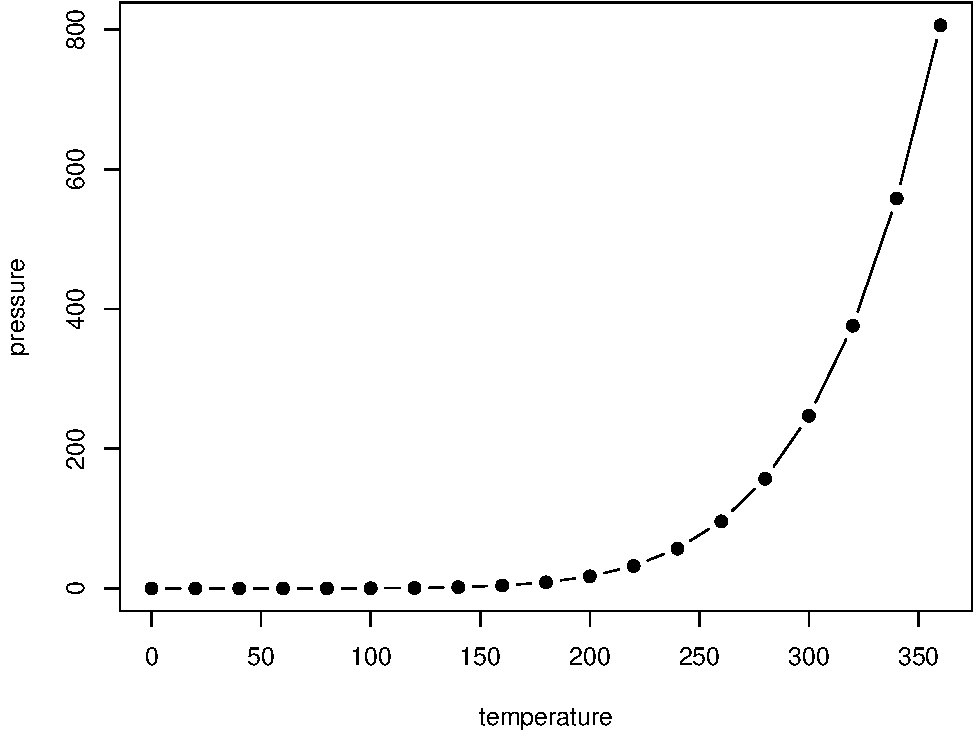
\includegraphics[width=0.8\linewidth]{healtheconomicsinR_files/figure-latex/nice-fig-1} 

}

\caption{Here is a nice figure!}\label{fig:nice-fig}
\end{figure}

Reference a figure by its code chunk label with the \texttt{fig:} prefix, e.g., see Figure \ref{fig:nice-fig}. Similarly, you can reference tables generated from \texttt{knitr::kable()}, e.g., see Table \ref{tab:nice-tab}.

\begin{Shaded}
\begin{Highlighting}[]
\NormalTok{knitr}\OperatorTok{::}\KeywordTok{kable}\NormalTok{(}
  \KeywordTok{head}\NormalTok{(iris, }\DecValTok{20}\NormalTok{), }\DataTypeTok{caption =} \StringTok{'Here is a nice table!'}\NormalTok{,}
  \DataTypeTok{booktabs =} \OtherTok{TRUE}
\NormalTok{)}
\end{Highlighting}
\end{Shaded}

\begin{table}[t]

\caption{\label{tab:nice-tab}Here is a nice table!}
\centering
\begin{tabular}{rrrrl}
\toprule
Sepal.Length & Sepal.Width & Petal.Length & Petal.Width & Species\\
\midrule
5.1 & 3.5 & 1.4 & 0.2 & setosa\\
4.9 & 3.0 & 1.4 & 0.2 & setosa\\
4.7 & 3.2 & 1.3 & 0.2 & setosa\\
4.6 & 3.1 & 1.5 & 0.2 & setosa\\
5.0 & 3.6 & 1.4 & 0.2 & setosa\\
\addlinespace
5.4 & 3.9 & 1.7 & 0.4 & setosa\\
4.6 & 3.4 & 1.4 & 0.3 & setosa\\
5.0 & 3.4 & 1.5 & 0.2 & setosa\\
4.4 & 2.9 & 1.4 & 0.2 & setosa\\
4.9 & 3.1 & 1.5 & 0.1 & setosa\\
\addlinespace
5.4 & 3.7 & 1.5 & 0.2 & setosa\\
4.8 & 3.4 & 1.6 & 0.2 & setosa\\
4.8 & 3.0 & 1.4 & 0.1 & setosa\\
4.3 & 3.0 & 1.1 & 0.1 & setosa\\
5.8 & 4.0 & 1.2 & 0.2 & setosa\\
\addlinespace
5.7 & 4.4 & 1.5 & 0.4 & setosa\\
5.4 & 3.9 & 1.3 & 0.4 & setosa\\
5.1 & 3.5 & 1.4 & 0.3 & setosa\\
5.7 & 3.8 & 1.7 & 0.3 & setosa\\
5.1 & 3.8 & 1.5 & 0.3 & setosa\\
\bottomrule
\end{tabular}
\end{table}

You can write citations, too. For example, we are using the \textbf{bookdown} package \citep{R-bookdown} in this sample book, which was built on top of R Markdown and \textbf{knitr} \citep{xie2015}.

\hypertarget{decisiontrees}{%
\chapter{Decision Trees}\label{decisiontrees}}

Introduction

\hypertarget{binary-trees}{%
\section{Binary Trees}\label{binary-trees}}

\hypertarget{sparcity}{%
\section{Sparcity}\label{sparcity}}

\hypertarget{dynamic-programming-and-bellman-equations}{%
\section{Dynamic Programming and Bellman Equations}\label{dynamic-programming-and-bellman-equations}}

\hypertarget{value-and-policy-iteration}{%
\subsection{Value and Policy Iteration}\label{value-and-policy-iteration}}

\hypertarget{discrete-event-simulation}{%
\chapter{Discrete Event Simulation}\label{discrete-event-simulation}}

Introduction

\hypertarget{priority-queues-and-stacks}{%
\section{(Priority) Queues and Stacks}\label{priority-queues-and-stacks}}

\hypertarget{push-and-pop}{%
\subsection{Push and Pop}\label{push-and-pop}}

\hypertarget{scheduler}{%
\section{Scheduler}\label{scheduler}}

\hypertarget{HRQoL}{%
\chapter{Health-realted Quality of Life}\label{HRQoL}}

Introduction

\hypertarget{qalys}{%
\section{QALYs}\label{qalys}}

\hypertarget{dalys}{%
\section{DALYs}\label{dalys}}

\hypertarget{combining-utilities}{%
\section{Combining Utilities}\label{combining-utilities}}

\hypertarget{markov-models}{%
\chapter{Markov Models}\label{markov-models}}

Introduction

\hypertarget{standard-matrix-formulation}{%
\section{Standard Matrix Formulation}\label{standard-matrix-formulation}}

\hypertarget{simulation}{%
\section{Simulation}\label{simulation}}

\hypertarget{C1}{%
\subsubsection{1. A simple decision tree}\label{C1}}

This example is taken from \citet{Hazen2014}.
The problem is concerned with a competing risk cancer and AIDS decision tree.
We will assume discrete time of single years.
An individual starts in the \texttt{Well} state.
They can transition into \texttt{Dead}, \texttt{Cancer\ \&\ AIDS}, \texttt{Cancer}, \texttt{AIDS} or remain in the \texttt{Well} state.

Define the transition probabilities:

\begin{itemize}
\tightlist
\item
  Die from other causes: \(\delta_0 = 0.001182\)
\item
  Die from recurent prostate cancer: \(\delta_c = 0.025\)
\item
  Die from AIDS: \(\delta_a = 0.080\)
\item
  Cancer recurs: \(\beta_c = 0.0027\)
\item
  Develop AIDS: \(\beta_a = 0.0083\)
\end{itemize}

Each state has an associated utility or benefit (quality factor in \citet{Hazen2014}) accrued by spending one cycle in each state.
Define the state utilities:

\begin{itemize}
\tightlist
\item
  \texttt{Well}: \(R_w=\) 1.0
\item
  \texttt{Cancer}: \(R_c=\) 0.60
\item
  \texttt{AIDS}: \(R_a=\) 0.50
\item
  \texttt{Cancer\ \&\ AIDS}: \(R_{ca}=\) 0.30
\item
  \texttt{Dead}: \(R_d=\) 0
\end{itemize}

Note that we will not include discounting.

C1. Define a (single year) decision tree and calculate the expected quality-adjusted value.

\hypertarget{C2}{%
\subsubsection{2. Markov-cycle tree}\label{C2}}

A Markov-cycle tree was introduced by \citet{Hollenberg1984} and is a representation of a Markov process in which the possible events taking place during each cycle are represented by a probability tree.
This is one way of simplifying determining probabilities from multiple paths.

The diagram for the Markov-cycle tree of the example in \citet{Hazen2014} is given below (note that the order of the states is different on the left-hand side and right-hand side).

\includegraphics[width=0.75\linewidth]{figs/markov_cycle_tree}

The terminal state are now root or source states, meaning the process returns to the left-hand side to be repeated.

C2. Extend the model of C1 for multiple cycles and thus create a Markov-cycle tree. Calculate the mean quality-adjusted lifetime of 90.473.

\hypertarget{C3}{%
\subsubsection{3. One-cycle Markov-cycle tree}\label{C3}}

We can rearrange the Markov-cycle tree to closer resemble a Markov model by collapsing the branches into a single cycle and simply combining the probabilities.

In the below figure

\begin{itemize}
\tightlist
\item
  The numbers above each branch are the one-cycle transition probabilities
\item
  The numbers pointing at nodes and names are the mean quality-adjusted durations accrued through \(n\) cycles.
\item
  The numbers in brackets are the mean quality-adjusted durations at the start of the cycle.
\end{itemize}

So for the below figure, the right-most numbers are the mean quality-adjusted durations for cycle 2, the left-most numbers are the mean quality-adjusted durations for cycle 3 and the numbers in brackets are the mean quality-adjusted durations for cycle 1.
\citet{Hazen2014} steps through this calculation in detail.

\includegraphics[width=0.65\linewidth]{figs/onecycle_markovcycletree}

C3. Modify the model of C2 to create a one-cycle Markov-cycle tree. Calculate the mean quality-adjusted lifetime.

\hypertarget{C4}{%
\subsubsection{4. Discrete-time Markov model}\label{C4}}

Clearly, the Markov-cycle tree can also be represented as a discrete-time Markov model.
The transition probabilities can be calculated by combining relevant path probabilities from the decision tree as done for the one-cycle Markov-cycle tree.
The model is shown below (note that death is not shows for simplicity).

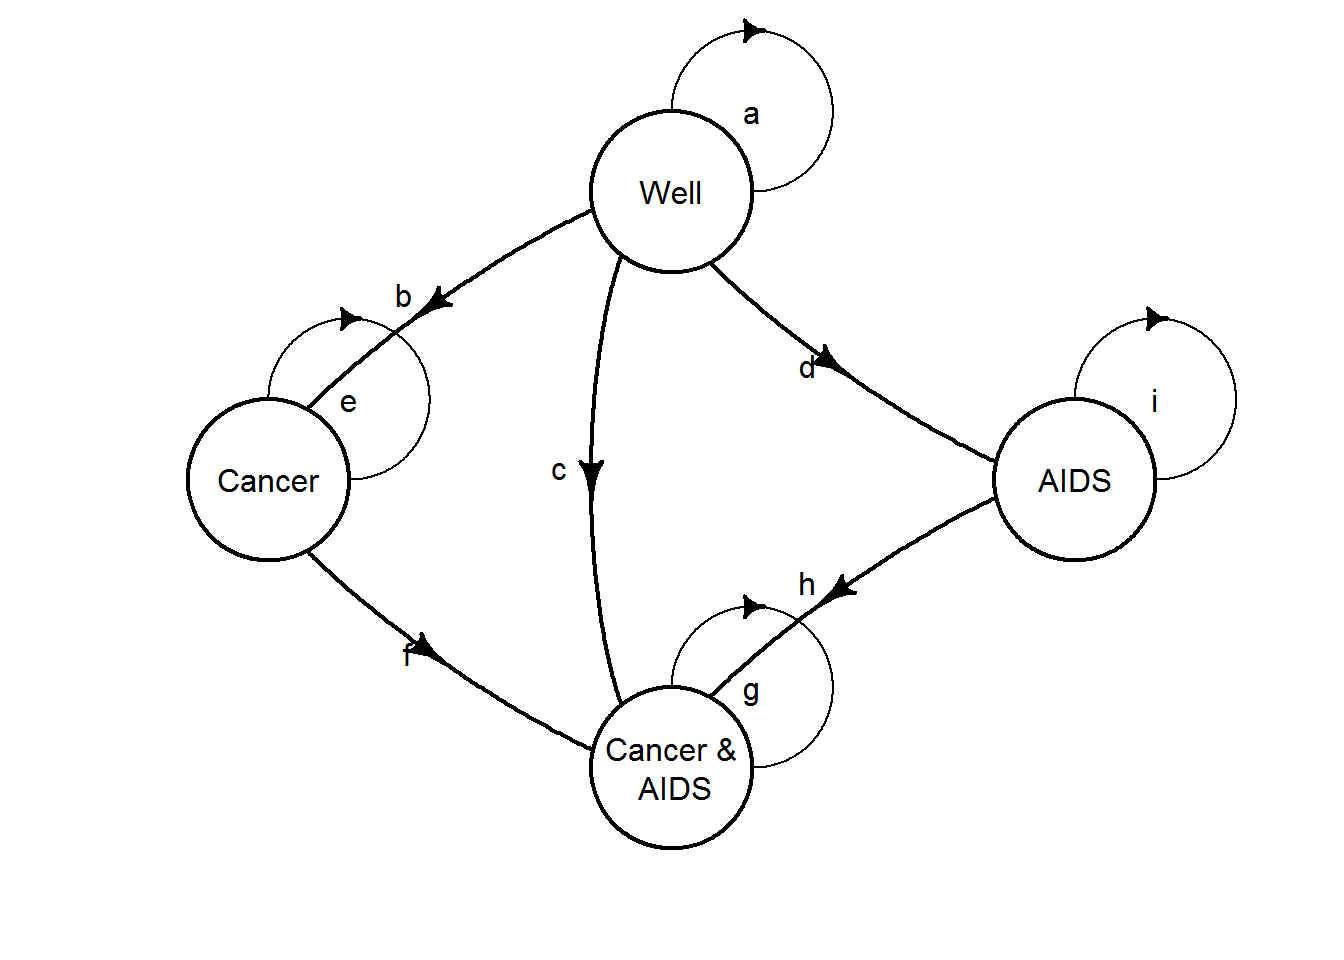
\includegraphics[width=0.75\linewidth]{healtheconomicsinR_files/figure-latex/unnamed-chunk-5-1}

C4. Create the equivalent discrete-time Markov model to the one-cycle Markov-cycle tree. Calculate cumulative proportion of patient cycles in each state and take product with health utilities for each respectively to obtain the mean quality-adjusted lifetime.

\hypertarget{C5}{%
\subsubsection{5. Roll back Markov-cycle tree}\label{C5}}

A neat strength is that we can calculate the mean quality-adjusted lifetime using the one-cycle Markov-cycle tree representation without calculating the cumulative proportion of time of patient cycles in each health state.
This is done by rolling back using the recursive equation (\href{https://en.wikipedia.org/wiki/Markov_decision_process\#Value_iteration}{value iteration}):

\[
V_n(i) = R(i) + \sum_j p_{ij} V_{n-1}(j)
\]
where \(V_n(i)\) are the values at node \(i\) at step \(n\), in our case the mean quality-adjusted lifetime.

C5. Calculate the mean quality-adjusted lifetime using the one-cycle Markov-cycle tree and value iteration.

\hypertarget{C6}{%
\subsubsection{6. (BONUS CHALLENGE): Roll back stochastic tree}\label{C6}}

So far we have only considered discrete time.
The Markov-cycle tree representation can be extended to continuous time as a \emph{stochastic tree}
(see \citet{Hazen2014} for details).
Probabilities are now replaced by rates.
This change is represented by zigzag lines in the diagrams.
This is clearly a more compact representation.

We can calculate mean quality-adjusted lifetime in an analogous way to the discrete-time case by rolling back using the recursive equation:

\[
V(S) = \frac{R(i)}{\sum_j \lambda_j} + \sum_j p_j V(S_j)
\]
The new model diagram is given below.

\includegraphics[width=0.75\linewidth]{figs/stochastic_tree}

The rates for state transitions are:

\begin{itemize}
\tightlist
\item
  \texttt{Cancer}: \(\lambda_c = 0.03250\)/year
\item
  \texttt{AIDS}: \(\lambda_a = 0.10\)/year
\item
  \texttt{Dead\ from\ Cancer}: \(\mu_c = 0.3081\)/year
\item
  \texttt{Dead\ from\ AIDS}: \(\mu_a = 0.9970\)/year
\item
  \texttt{Dead\ other}: \(\mu_o = 0.014191\)/year
\end{itemize}

C6. Create the stochastic tree model and calculate the mean quality-adjusted lifetime using value iteration.

~

\hypertarget{references}{%
\subsection{References}\label{references}}

Load supporting packages.

\begin{Shaded}
\begin{Highlighting}[]
\KeywordTok{library}\NormalTok{(purrr)}
\KeywordTok{library}\NormalTok{(knitr)}
\end{Highlighting}
\end{Shaded}

\hypertarget{c1.-a-simple-decision-tree}{%
\subsubsection{C1. A simple decision tree}\label{c1.-a-simple-decision-tree}}

Define the separate monthly transition probabilities.

\begin{Shaded}
\begin{Highlighting}[]
\NormalTok{delta0 <-}\StringTok{ }\FloatTok{0.001182}
\NormalTok{deltac <-}\StringTok{ }\FloatTok{0.025}
\NormalTok{deltaa <-}\StringTok{ }\FloatTok{0.08}
\NormalTok{betac  <-}\StringTok{ }\FloatTok{0.0027}
\NormalTok{betaa  <-}\StringTok{ }\FloatTok{0.0083}
\end{Highlighting}
\end{Shaded}

and the utilities of being in each state.

\begin{Shaded}
\begin{Highlighting}[]
\NormalTok{sutils <-}\StringTok{ }\KeywordTok{c}\NormalTok{(}\DataTypeTok{dead =} \DecValTok{0}\NormalTok{, }\DataTypeTok{CA =} \FloatTok{0.3}\NormalTok{, }\DataTypeTok{cancer =} \FloatTok{0.6}\NormalTok{, }\DataTypeTok{AIDS =} \FloatTok{0.5}\NormalTok{, }\DataTypeTok{well =} \DecValTok{1}\NormalTok{)}
\end{Highlighting}
\end{Shaded}

Note that the order of states is \texttt{dead}, \texttt{cancer\ \&\ AIDS}, \texttt{cancer}, \texttt{AIDS}, \texttt{well}.

Define decision trees in terms of the structure, values and probabilities.
We'll use the \texttt{tribble} function just because it allows us to specify a matrix by rows rather than columns.

\begin{Shaded}
\begin{Highlighting}[]
\KeywordTok{library}\NormalTok{(tibble)}

\NormalTok{tree_probs <-}\StringTok{ }\KeywordTok{list}\NormalTok{()}

\CommentTok{# unique state outcomes each branch}
\NormalTok{tree_probs}\OperatorTok{$}\NormalTok{well <-}
\StringTok{  }\KeywordTok{tribble}\NormalTok{(}\OperatorTok{~}\NormalTok{rowname,  }\OperatorTok{~}\NormalTok{dead, }\OperatorTok{~}\NormalTok{ndead,  }\OperatorTok{~}\NormalTok{recurc, }\OperatorTok{~}\NormalTok{ncancer, }\OperatorTok{~}\NormalTok{CA,  }\OperatorTok{~}\NormalTok{cancer, }\OperatorTok{~}\NormalTok{AIDS, }\OperatorTok{~}\NormalTok{well,}
          \StringTok{"well0"}\NormalTok{,   delta0,}\DecValTok{1}\OperatorTok{-}\NormalTok{delta0,}\OtherTok{NA}\NormalTok{,      }\OtherTok{NA}\NormalTok{,       }\OtherTok{NA}\NormalTok{,   }\OtherTok{NA}\NormalTok{,      }\OtherTok{NA}\NormalTok{,    }\OtherTok{NA}\NormalTok{,}
          \StringTok{"ndead"}\NormalTok{,   }\OtherTok{NA}\NormalTok{,    }\OtherTok{NA}\NormalTok{,      betac,   }\DecValTok{1}\OperatorTok{-}\NormalTok{betac,  }\OtherTok{NA}\NormalTok{,   }\OtherTok{NA}\NormalTok{,      }\OtherTok{NA}\NormalTok{,    }\OtherTok{NA}\NormalTok{,}
          \StringTok{"recurc"}\NormalTok{,  }\OtherTok{NA}\NormalTok{,    }\OtherTok{NA}\NormalTok{,      }\OtherTok{NA}\NormalTok{,      }\OtherTok{NA}\NormalTok{,       betaa,}\DecValTok{1}\OperatorTok{-}\NormalTok{betaa, }\OtherTok{NA}\NormalTok{,    }\OtherTok{NA}\NormalTok{,}
          \StringTok{"ncancer"}\NormalTok{, }\OtherTok{NA}\NormalTok{,    }\OtherTok{NA}\NormalTok{,      }\OtherTok{NA}\NormalTok{,      }\OtherTok{NA}\NormalTok{,       }\OtherTok{NA}\NormalTok{,   }\OtherTok{NA}\NormalTok{,      betaa, }\DecValTok{1}\OperatorTok{-}\NormalTok{betaa) }\OperatorTok\StringTok{ }
\StringTok{  }\KeywordTok{column_to_rownames}\NormalTok{()}

\NormalTok{tree_probs}\OperatorTok{$}\NormalTok{cancer <-}
\StringTok{  }\KeywordTok{tribble}\NormalTok{(}\OperatorTok{~}\NormalTok{rowname, }\OperatorTok{~}\NormalTok{dead, }\OperatorTok{~}\NormalTok{ndead,  }\OperatorTok{~}\NormalTok{diec, }\OperatorTok{~}\NormalTok{survc,  }\OperatorTok{~}\NormalTok{CA,  }\OperatorTok{~}\NormalTok{cancer,}
          \StringTok{"cancer0"}\NormalTok{,delta0,}\DecValTok{1}\OperatorTok{-}\NormalTok{delta0,}\OtherTok{NA}\NormalTok{,    }\OtherTok{NA}\NormalTok{,      }\OtherTok{NA}\NormalTok{,   }\OtherTok{NA}\NormalTok{,}
          \StringTok{"ndead"}\NormalTok{,  }\OtherTok{NA}\NormalTok{,    }\OtherTok{NA}\NormalTok{,      deltac,}\DecValTok{1}\OperatorTok{-}\NormalTok{deltac,}\OtherTok{NA}\NormalTok{,   }\OtherTok{NA}\NormalTok{,}
          \StringTok{"survc"}\NormalTok{,  }\OtherTok{NA}\NormalTok{,    }\OtherTok{NA}\NormalTok{,      }\OtherTok{NA}\NormalTok{,    }\OtherTok{NA}\NormalTok{,      betaa,}\DecValTok{1}\OperatorTok{-}\NormalTok{betaa) }\OperatorTok\StringTok{ }
\StringTok{  }\KeywordTok{column_to_rownames}\NormalTok{()}

\NormalTok{tree_probs}\OperatorTok{$}\NormalTok{AIDS <-}
\StringTok{  }\KeywordTok{tribble}\NormalTok{(}\OperatorTok{~}\NormalTok{rowname,}\OperatorTok{~}\NormalTok{dead, }\OperatorTok{~}\NormalTok{ndead,  }\OperatorTok{~}\NormalTok{diea, }\OperatorTok{~}\NormalTok{surva,  }\OperatorTok{~}\NormalTok{CA,  }\OperatorTok{~}\NormalTok{AIDS,}
          \StringTok{"AIDS0"}\NormalTok{, delta0,}\DecValTok{1}\OperatorTok{-}\NormalTok{delta0,}\OtherTok{NA}\NormalTok{,    }\OtherTok{NA}\NormalTok{,      }\OtherTok{NA}\NormalTok{,   }\OtherTok{NA}\NormalTok{,}
          \StringTok{"ndead"}\NormalTok{, }\OtherTok{NA}\NormalTok{,    }\OtherTok{NA}\NormalTok{,      deltaa,}\DecValTok{1}\OperatorTok{-}\NormalTok{deltaa,}\OtherTok{NA}\NormalTok{,   }\OtherTok{NA}\NormalTok{,}
          \StringTok{"surva"}\NormalTok{, }\OtherTok{NA}\NormalTok{,    }\OtherTok{NA}\NormalTok{,      }\OtherTok{NA}\NormalTok{,    }\OtherTok{NA}\NormalTok{,      betac,}\DecValTok{1}\OperatorTok{-}\NormalTok{betac) }\OperatorTok\StringTok{ }
\StringTok{  }\KeywordTok{column_to_rownames}\NormalTok{()}

\NormalTok{tree_probs}\OperatorTok{$}\NormalTok{CA <-}
\StringTok{  }\KeywordTok{tribble}\NormalTok{(}\OperatorTok{~}\NormalTok{rowname,}\OperatorTok{~}\NormalTok{dead, }\OperatorTok{~}\NormalTok{ndead,  }\OperatorTok{~}\NormalTok{diec, }\OperatorTok{~}\NormalTok{survc,  }\OperatorTok{~}\NormalTok{diea, }\OperatorTok{~}\NormalTok{CA,}
          \StringTok{"CA0"}\NormalTok{,   delta0,}\DecValTok{1}\OperatorTok{-}\NormalTok{delta0,}\OtherTok{NA}\NormalTok{,    }\OtherTok{NA}\NormalTok{,      }\OtherTok{NA}\NormalTok{,    }\OtherTok{NA}\NormalTok{,}
          \StringTok{"ndead"}\NormalTok{, }\OtherTok{NA}\NormalTok{,    }\OtherTok{NA}\NormalTok{,      deltac,}\DecValTok{1}\OperatorTok{-}\NormalTok{deltac,}\OtherTok{NA}\NormalTok{,    }\OtherTok{NA}\NormalTok{,}
          \StringTok{"survc"}\NormalTok{, }\OtherTok{NA}\NormalTok{,    }\OtherTok{NA}\NormalTok{,      }\OtherTok{NA}\NormalTok{,    }\OtherTok{NA}\NormalTok{,      deltaa,}\DecValTok{1}\OperatorTok{-}\NormalTok{deltaa) }\OperatorTok\StringTok{ }
\StringTok{  }\KeywordTok{column_to_rownames}\NormalTok{()}

\NormalTok{tree_probs}\OperatorTok{$}\NormalTok{dead <-}\StringTok{ }\DecValTok{1}

\NormalTok{tree_probs}
\end{Highlighting}
\end{Shaded}

\begin{verbatim}
## $well
##             dead    ndead recurc ncancer     CA cancer   AIDS   well
## well0   0.001182 0.998818     NA      NA     NA     NA     NA     NA
## ndead         NA       NA 0.0027  0.9973     NA     NA     NA     NA
## recurc        NA       NA     NA      NA 0.0083 0.9917     NA     NA
## ncancer       NA       NA     NA      NA     NA     NA 0.0083 0.9917
## 
## $cancer
##             dead    ndead  diec survc     CA cancer
## cancer0 0.001182 0.998818    NA    NA     NA     NA
## ndead         NA       NA 0.025 0.975     NA     NA
## survc         NA       NA    NA    NA 0.0083 0.9917
## 
## $AIDS
##           dead    ndead diea surva     CA   AIDS
## AIDS0 0.001182 0.998818   NA    NA     NA     NA
## ndead       NA       NA 0.08  0.92     NA     NA
## surva       NA       NA   NA    NA 0.0027 0.9973
## 
## $CA
##           dead    ndead  diec survc diea   CA
## CA0   0.001182 0.998818    NA    NA   NA   NA
## ndead       NA       NA 0.025 0.975   NA   NA
## survc       NA       NA    NA    NA 0.08 0.92
## 
## $dead
## [1] 1
\end{verbatim}

\begin{Shaded}
\begin{Highlighting}[]
\NormalTok{tree_vals <-}\StringTok{ }\KeywordTok{list}\NormalTok{()}

\NormalTok{tree_vals}\OperatorTok{$}\NormalTok{well <-}
\StringTok{  }\KeywordTok{tribble}\NormalTok{(}\OperatorTok{~}\NormalTok{rowname, }\OperatorTok{~}\NormalTok{dead, }\OperatorTok{~}\NormalTok{ndead, }\OperatorTok{~}\NormalTok{cancer, }\OperatorTok{~}\NormalTok{ncancer, }\OperatorTok{~}\NormalTok{CA, }\OperatorTok{~}\NormalTok{CnotA, }\OperatorTok{~}\NormalTok{AIDS, }\OperatorTok{~}\NormalTok{well,}
          \StringTok{"well0"}\NormalTok{, }\DecValTok{0}\NormalTok{,}\DecValTok{0}\NormalTok{,}\DecValTok{0}\NormalTok{,}\DecValTok{0}\NormalTok{,}\DecValTok{0}\NormalTok{,}\DecValTok{0}\NormalTok{,}\DecValTok{0}\NormalTok{,}\DecValTok{0}\NormalTok{,}
          \StringTok{"ndead"}\NormalTok{, }\DecValTok{0}\NormalTok{,}\DecValTok{0}\NormalTok{,}\DecValTok{0}\NormalTok{,}\DecValTok{0}\NormalTok{,}\DecValTok{0}\NormalTok{,}\DecValTok{0}\NormalTok{,}\DecValTok{0}\NormalTok{,}\DecValTok{0}\NormalTok{,}
          \StringTok{"cancer"}\NormalTok{, }\DecValTok{0}\NormalTok{,}\DecValTok{0}\NormalTok{,}\DecValTok{0}\NormalTok{,}\DecValTok{0}\NormalTok{,}\FloatTok{0.3}\NormalTok{,}\FloatTok{0.6}\NormalTok{,}\DecValTok{0}\NormalTok{,}\DecValTok{0}\NormalTok{,}
          \StringTok{"ncancer"}\NormalTok{, }\DecValTok{0}\NormalTok{,}\DecValTok{0}\NormalTok{,}\DecValTok{0}\NormalTok{,}\DecValTok{0}\NormalTok{,}\DecValTok{0}\NormalTok{,}\DecValTok{0}\NormalTok{,}\FloatTok{0.5}\NormalTok{,}\DecValTok{1}\NormalTok{) }\OperatorTok\StringTok{ }
\StringTok{  }\KeywordTok{column_to_rownames}\NormalTok{()}

\NormalTok{tree_vals}\OperatorTok{$}\NormalTok{cancer <-}
\StringTok{  }\KeywordTok{tribble}\NormalTok{(}\OperatorTok{~}\NormalTok{rowname, }\OperatorTok{~}\NormalTok{dead, }\OperatorTok{~}\NormalTok{ndead, }\OperatorTok{~}\NormalTok{cancer, }\OperatorTok{~}\NormalTok{ncancer, }\OperatorTok{~}\NormalTok{CA, }\OperatorTok{~}\NormalTok{CnotA, }\OperatorTok{~}\NormalTok{AIDS, }\OperatorTok{~}\NormalTok{well,}
          \StringTok{"well"}\NormalTok{, }\DecValTok{0}\NormalTok{,}\DecValTok{0}\NormalTok{,}\DecValTok{0}\NormalTok{,}\DecValTok{0}\NormalTok{,}\DecValTok{0}\NormalTok{,}\DecValTok{0}\NormalTok{,}\DecValTok{0}\NormalTok{,}\DecValTok{0}\NormalTok{,}
          \StringTok{"ndead"}\NormalTok{, }\DecValTok{0}\NormalTok{,}\DecValTok{0}\NormalTok{,}\DecValTok{0}\NormalTok{,}\DecValTok{0}\NormalTok{,}\DecValTok{0}\NormalTok{,}\DecValTok{0}\NormalTok{,}\DecValTok{0}\NormalTok{,}\DecValTok{0}\NormalTok{,}
          \StringTok{"cancer"}\NormalTok{, }\DecValTok{0}\NormalTok{,}\DecValTok{0}\NormalTok{,}\DecValTok{0}\NormalTok{,}\DecValTok{0}\NormalTok{,}\FloatTok{0.3}\NormalTok{,}\FloatTok{0.6}\NormalTok{,}\DecValTok{0}\NormalTok{,}\DecValTok{0}\NormalTok{,}
          \StringTok{"ncancer"}\NormalTok{, }\DecValTok{0}\NormalTok{,}\DecValTok{0}\NormalTok{,}\DecValTok{0}\NormalTok{,}\DecValTok{0}\NormalTok{,}\DecValTok{0}\NormalTok{,}\DecValTok{0}\NormalTok{,}\FloatTok{0.5}\NormalTok{,}\DecValTok{1}\NormalTok{) }\OperatorTok\StringTok{ }
\StringTok{  }\KeywordTok{column_to_rownames}\NormalTok{()}

\NormalTok{tree_vals}\OperatorTok{$}\NormalTok{AIDS <-}
\StringTok{  }\KeywordTok{tribble}\NormalTok{(}\OperatorTok{~}\NormalTok{rowname, }\OperatorTok{~}\NormalTok{dead, }\OperatorTok{~}\NormalTok{ndead, }\OperatorTok{~}\NormalTok{cancer, }\OperatorTok{~}\NormalTok{ncancer, }\OperatorTok{~}\NormalTok{CA, }\OperatorTok{~}\NormalTok{CnotA, }\OperatorTok{~}\NormalTok{AIDS, }\OperatorTok{~}\NormalTok{well,}
          \StringTok{"well"}\NormalTok{, }\DecValTok{0}\NormalTok{,}\DecValTok{0}\NormalTok{,}\DecValTok{0}\NormalTok{,}\DecValTok{0}\NormalTok{,}\DecValTok{0}\NormalTok{,}\DecValTok{0}\NormalTok{,}\DecValTok{0}\NormalTok{,}\DecValTok{0}\NormalTok{,}
          \StringTok{"ndead"}\NormalTok{, }\DecValTok{0}\NormalTok{,}\DecValTok{0}\NormalTok{,}\DecValTok{0}\NormalTok{,}\DecValTok{0}\NormalTok{,}\DecValTok{0}\NormalTok{,}\DecValTok{0}\NormalTok{,}\DecValTok{0}\NormalTok{,}\DecValTok{0}\NormalTok{,}
          \StringTok{"cancer"}\NormalTok{, }\DecValTok{0}\NormalTok{,}\DecValTok{0}\NormalTok{,}\DecValTok{0}\NormalTok{,}\DecValTok{0}\NormalTok{,}\FloatTok{0.3}\NormalTok{,}\FloatTok{0.6}\NormalTok{,}\DecValTok{0}\NormalTok{,}\DecValTok{0}\NormalTok{,}
          \StringTok{"ncancer"}\NormalTok{, }\DecValTok{0}\NormalTok{,}\DecValTok{0}\NormalTok{,}\DecValTok{0}\NormalTok{,}\DecValTok{0}\NormalTok{,}\DecValTok{0}\NormalTok{,}\DecValTok{0}\NormalTok{,}\FloatTok{0.5}\NormalTok{,}\DecValTok{1}\NormalTok{) }\OperatorTok\StringTok{ }
\StringTok{  }\KeywordTok{column_to_rownames}\NormalTok{()}

\NormalTok{tree_vals}\OperatorTok{$}\NormalTok{CA <-}
\StringTok{  }\KeywordTok{tribble}\NormalTok{(}\OperatorTok{~}\NormalTok{rowname, }\OperatorTok{~}\NormalTok{dead, }\OperatorTok{~}\NormalTok{ndead, }\OperatorTok{~}\NormalTok{cancer, }\OperatorTok{~}\NormalTok{ncancer, }\OperatorTok{~}\NormalTok{CA, }\OperatorTok{~}\NormalTok{CnotA, }\OperatorTok{~}\NormalTok{AIDS, }\OperatorTok{~}\NormalTok{well,}
          \StringTok{"well"}\NormalTok{, }\DecValTok{0}\NormalTok{,}\DecValTok{0}\NormalTok{,}\DecValTok{0}\NormalTok{,}\DecValTok{0}\NormalTok{,}\DecValTok{0}\NormalTok{,}\DecValTok{0}\NormalTok{,}\DecValTok{0}\NormalTok{,}\DecValTok{0}\NormalTok{,}
          \StringTok{"ndead"}\NormalTok{, }\DecValTok{0}\NormalTok{,}\DecValTok{0}\NormalTok{,}\DecValTok{0}\NormalTok{,}\DecValTok{0}\NormalTok{,}\DecValTok{0}\NormalTok{,}\DecValTok{0}\NormalTok{,}\DecValTok{0}\NormalTok{,}\DecValTok{0}\NormalTok{,}
          \StringTok{"cancer"}\NormalTok{, }\DecValTok{0}\NormalTok{,}\DecValTok{0}\NormalTok{,}\DecValTok{0}\NormalTok{,}\DecValTok{0}\NormalTok{,}\FloatTok{0.3}\NormalTok{,}\FloatTok{0.6}\NormalTok{,}\DecValTok{0}\NormalTok{,}\DecValTok{0}\NormalTok{,}
          \StringTok{"ncancer"}\NormalTok{, }\DecValTok{0}\NormalTok{,}\DecValTok{0}\NormalTok{,}\DecValTok{0}\NormalTok{,}\DecValTok{0}\NormalTok{,}\DecValTok{0}\NormalTok{,}\DecValTok{0}\NormalTok{,}\FloatTok{0.5}\NormalTok{,}\DecValTok{1}\NormalTok{) }\OperatorTok\StringTok{ }
\StringTok{  }\KeywordTok{column_to_rownames}\NormalTok{()}
\end{Highlighting}
\end{Shaded}

\hypertarget{c2.-extend-c1-for-multiple-cycles}{%
\subsubsection{C2. Extend C1 for multiple cycles}\label{c2.-extend-c1-for-multiple-cycles}}

Assuming a binomial tree we can forward simulate for a synthetic cohort. This is a brute force approach and is potentially time-consuming.

\begin{Shaded}
\begin{Highlighting}[]
\NormalTok{cohort <-}\StringTok{ }\KeywordTok{list}\NormalTok{()}
\NormalTok{n_cohort <-}\StringTok{ }\DecValTok{1000}
\NormalTok{death_states <-}\StringTok{ }\KeywordTok{c}\NormalTok{(}\StringTok{"diea"}\NormalTok{, }\StringTok{"diec"}\NormalTok{, }\StringTok{"dead"}\NormalTok{)}

\ControlFlowTok{for}\NormalTok{ (i }\ControlFlowTok{in} \KeywordTok{seq_len}\NormalTok{(n_cohort)) \{}
  
\NormalTok{  traj_s <-}\StringTok{ }\OtherTok{NULL}
\NormalTok{  traj_u <-}\StringTok{ }\OtherTok{NULL}
\NormalTok{  state_name <-}\StringTok{ "well"}
  
  \ControlFlowTok{while}\NormalTok{ (}\OperatorTok{!}\NormalTok{state_name }\OperatorTok\StringTok{ }\NormalTok{death_states) \{}
    
\NormalTok{    p <-}\StringTok{ }\NormalTok{tree_probs[[state_name]]}
\NormalTok{    binp <-}\StringTok{ }\NormalTok{p[state_name, }\OperatorTok{!}\KeywordTok{is.na}\NormalTok{(p[state_name, ])] }\CommentTok{#partial match}
    
    \ControlFlowTok{while}\NormalTok{ (}\KeywordTok{nrow}\NormalTok{(binp) }\OperatorTok{>}\StringTok{ }\DecValTok{0}\NormalTok{) \{}
      
\NormalTok{      state_name <-}\StringTok{ }
\StringTok{        }\ControlFlowTok{if}\NormalTok{ (}\KeywordTok{runif}\NormalTok{(}\DecValTok{1}\NormalTok{) }\OperatorTok{<}\StringTok{ }\NormalTok{binp[}\DecValTok{1}\NormalTok{]) }\KeywordTok{names}\NormalTok{(binp)[}\DecValTok{1}\NormalTok{] }\ControlFlowTok{else} \KeywordTok{names}\NormalTok{(binp)[}\DecValTok{2}\NormalTok{]}
      
\NormalTok{      binp <-}\StringTok{ }\NormalTok{p[state_name }\OperatorTok{==}\StringTok{ }\KeywordTok{rownames}\NormalTok{(p), }\OperatorTok{!}\KeywordTok{is.na}\NormalTok{(p[state_name, ])]}
\NormalTok{    \}}
    
\NormalTok{    traj_s <-}\StringTok{ }\KeywordTok{c}\NormalTok{(traj_s, state_name)}
\NormalTok{    traj_u <-}\StringTok{ }\KeywordTok{c}\NormalTok{(traj_u, sutils[state_name])}
\NormalTok{  \}}
  
\NormalTok{  cohort[[i]] <-}\StringTok{ }\NormalTok{traj_u }
\NormalTok{\}}
\end{Highlighting}
\end{Shaded}

An example trajectory

\begin{Shaded}
\begin{Highlighting}[]
\NormalTok{cohort[[}\DecValTok{1}\NormalTok{]]}
\end{Highlighting}
\end{Shaded}

\begin{verbatim}
## well well well well well well well well well well well well well well well 
##  1.0  1.0  1.0  1.0  1.0  1.0  1.0  1.0  1.0  1.0  1.0  1.0  1.0  1.0  1.0 
## well well well well well well well well well well well well well well well 
##  1.0  1.0  1.0  1.0  1.0  1.0  1.0  1.0  1.0  1.0  1.0  1.0  1.0  1.0  1.0 
## well well well well well well well well well well well well well well well 
##  1.0  1.0  1.0  1.0  1.0  1.0  1.0  1.0  1.0  1.0  1.0  1.0  1.0  1.0  1.0 
## well well well well well well well well well well well well well well well 
##  1.0  1.0  1.0  1.0  1.0  1.0  1.0  1.0  1.0  1.0  1.0  1.0  1.0  1.0  1.0 
## well well well well well well well well well well well well well well well 
##  1.0  1.0  1.0  1.0  1.0  1.0  1.0  1.0  1.0  1.0  1.0  1.0  1.0  1.0  1.0 
## well well well well well well well well well well well well well well well 
##  1.0  1.0  1.0  1.0  1.0  1.0  1.0  1.0  1.0  1.0  1.0  1.0  1.0  1.0  1.0 
## well well well well well well well well well well well well well well well 
##  1.0  1.0  1.0  1.0  1.0  1.0  1.0  1.0  1.0  1.0  1.0  1.0  1.0  1.0  1.0 
## well well well well well well well well well well well well well well well 
##  1.0  1.0  1.0  1.0  1.0  1.0  1.0  1.0  1.0  1.0  1.0  1.0  1.0  1.0  1.0 
## well well well well well well well well well well well well well well well 
##  1.0  1.0  1.0  1.0  1.0  1.0  1.0  1.0  1.0  1.0  1.0  1.0  1.0  1.0  1.0 
## well well well well well well well well well well well well well well well 
##  1.0  1.0  1.0  1.0  1.0  1.0  1.0  1.0  1.0  1.0  1.0  1.0  1.0  1.0  1.0 
## well well well well well well well well well well well AIDS AIDS AIDS AIDS 
##  1.0  1.0  1.0  1.0  1.0  1.0  1.0  1.0  1.0  1.0  1.0  0.5  0.5  0.5  0.5 
## AIDS AIDS AIDS AIDS AIDS AIDS AIDS AIDS AIDS AIDS AIDS <NA> 
##  0.5  0.5  0.5  0.5  0.5  0.5  0.5  0.5  0.5  0.5  0.5   NA
\end{verbatim}

The mean summary statistics should be close to the true expected value.
However, it appears to be pretty noisy and even for fairly large values (in terms of run time) it can be off by one or two.

\begin{Shaded}
\begin{Highlighting}[]
\KeywordTok{mean}\NormalTok{(}\KeywordTok{map}\NormalTok{(cohort, sum, }\DataTypeTok{na.rm =} \OtherTok{TRUE}\NormalTok{) }\OperatorTok\StringTok{ }\KeywordTok{unlist}\NormalTok{())}
\end{Highlighting}
\end{Shaded}

\begin{verbatim}
## [1] 88.0646
\end{verbatim}

\hypertarget{c3.-markov-cycle-tree}{%
\subsubsection{C3. Markov-cycle tree}\label{c3.-markov-cycle-tree}}

Given the following transition matrix

\[
\tiny
\left(
\begin{matrix}
1 & 0 & 0 & 0 & 0\\
(1 - \delta_0)\delta_c + (1-\delta_0)(1-\delta_c)\delta_a & (1-\delta_0)(1-\delta_c(1-\delta_a) & 0 & 0 & 0\\
\delta_0 + (1-\delta_0)\delta_c & (1-\delta_0)(1-\delta_c)\beta_a & (1-\delta_0)(1-\delta_c)(1-\beta_a) & 0 & 0\\
\delta_0 + (1-\delta_0)\delta_a & (1-\delta_0)\beta_c(1-\delta_a) & 0 & (1-\delta_0)(1-\beta_c)(1-\delta_a) & 0\\
\delta_0 & (1-\delta_0)\beta_c\beta_a & (1-\delta_0)\beta_c(1-\beta_a) & (1-\delta_0)(1-\beta_c)\beta_a & (1-\delta_0)(1-\beta_c)(1-\beta_a)
\end{matrix}
\right)
\]

Then define the transition matrix object

\begin{Shaded}
\begin{Highlighting}[]
\NormalTok{p <-}\StringTok{ }\KeywordTok{list}\NormalTok{()}

\NormalTok{p}\OperatorTok{$}\NormalTok{dead <-}\StringTok{ }\KeywordTok{c}\NormalTok{(}\DecValTok{1}\NormalTok{,}\DecValTok{0}\NormalTok{,}\DecValTok{0}\NormalTok{,}\DecValTok{0}\NormalTok{,}\DecValTok{0}\NormalTok{)}

\NormalTok{p}\OperatorTok{$}\NormalTok{CA <-}
\StringTok{  }\KeywordTok{c}\NormalTok{(delta0 }\OperatorTok{+}\StringTok{ }\NormalTok{(}\DecValTok{1}\OperatorTok{-}\NormalTok{delta0)}\OperatorTok{*}\NormalTok{deltac }\OperatorTok{+}\StringTok{ }\NormalTok{(}\DecValTok{1}\OperatorTok{-}\NormalTok{delta0)}\OperatorTok{*}\NormalTok{(}\DecValTok{1}\OperatorTok{-}\NormalTok{deltac)}\OperatorTok{*}\NormalTok{deltaa, (}\DecValTok{1}\OperatorTok{-}\NormalTok{delta0)}\OperatorTok{*}\NormalTok{(}\DecValTok{1}\OperatorTok{-}\NormalTok{deltac)}\OperatorTok{*}\NormalTok{(}\DecValTok{1}\OperatorTok{-}\NormalTok{deltaa),}\DecValTok{0}\NormalTok{,}\DecValTok{0}\NormalTok{,}\DecValTok{0}\NormalTok{)}

\NormalTok{p}\OperatorTok{$}\NormalTok{cancer <-}
\StringTok{  }\KeywordTok{c}\NormalTok{(delta0 }\OperatorTok{+}\StringTok{ }\NormalTok{(}\DecValTok{1}\OperatorTok{-}\NormalTok{delta0)}\OperatorTok{*}\NormalTok{deltac, (}\DecValTok{1}\OperatorTok{-}\NormalTok{delta0)}\OperatorTok{*}\NormalTok{(}\DecValTok{1}\OperatorTok{-}\NormalTok{deltac)}\OperatorTok{*}\NormalTok{betaa, (}\DecValTok{1}\OperatorTok{-}\NormalTok{delta0)}\OperatorTok{*}\NormalTok{(}\DecValTok{1}\OperatorTok{-}\NormalTok{deltac)}\OperatorTok{*}\NormalTok{(}\DecValTok{1}\OperatorTok{-}\NormalTok{betaa),}\DecValTok{0}\NormalTok{,}\DecValTok{0}\NormalTok{)}

\NormalTok{p}\OperatorTok{$}\NormalTok{AIDS <-}
\StringTok{  }\KeywordTok{c}\NormalTok{(delta0 }\OperatorTok{+}\StringTok{ }\NormalTok{(}\DecValTok{1}\OperatorTok{-}\NormalTok{delta0)}\OperatorTok{*}\NormalTok{deltaa, (}\DecValTok{1}\OperatorTok{-}\NormalTok{delta0)}\OperatorTok{*}\NormalTok{betac}\OperatorTok{*}\NormalTok{(}\DecValTok{1}\OperatorTok{-}\NormalTok{deltaa), }\DecValTok{0}\NormalTok{, (}\DecValTok{1}\OperatorTok{-}\NormalTok{delta0)}\OperatorTok{*}\NormalTok{(}\DecValTok{1}\OperatorTok{-}\NormalTok{betac)}\OperatorTok{*}\NormalTok{(}\DecValTok{1}\OperatorTok{-}\NormalTok{deltaa), }\DecValTok{0}\NormalTok{)}

\NormalTok{p}\OperatorTok{$}\NormalTok{well <-}
\StringTok{  }\KeywordTok{c}\NormalTok{(delta0, (}\DecValTok{1}\OperatorTok{-}\NormalTok{delta0)}\OperatorTok{*}\NormalTok{betac}\OperatorTok{*}\NormalTok{betaa, (}\DecValTok{1}\OperatorTok{-}\NormalTok{delta0)}\OperatorTok{*}\NormalTok{betac}\OperatorTok{*}\NormalTok{(}\DecValTok{1}\OperatorTok{-}\NormalTok{betaa), (}\DecValTok{1}\OperatorTok{-}\NormalTok{delta0)}\OperatorTok{*}\NormalTok{(}\DecValTok{1}\OperatorTok{-}\NormalTok{betac)}\OperatorTok{*}\NormalTok{betaa,}
\NormalTok{    (}\DecValTok{1}\OperatorTok{-}\NormalTok{delta0)}\OperatorTok{*}\NormalTok{(}\DecValTok{1}\OperatorTok{-}\NormalTok{betac)}\OperatorTok{*}\NormalTok{(}\DecValTok{1}\OperatorTok{-}\NormalTok{betaa))}

\NormalTok{trans <-}\StringTok{ }\KeywordTok{do.call}\NormalTok{(rbind, p)}
\end{Highlighting}
\end{Shaded}

Combine the tree data all together into a single list using a function.

\begin{Shaded}
\begin{Highlighting}[]
\NormalTok{create_tree <-}\StringTok{ }\ControlFlowTok{function}\NormalTok{(trans, utils) \{}
  
  \ControlFlowTok{if}\NormalTok{ (}\OperatorTok{!}\KeywordTok{all}\NormalTok{(}\KeywordTok{rowSums}\NormalTok{(trans) }\OperatorTok{==}\StringTok{ }\DecValTok{1}\NormalTok{)) }\KeywordTok{stop}\NormalTok{(}\StringTok{"probabilities don't sum to one"}\NormalTok{)}
  \ControlFlowTok{if}\NormalTok{ (}\KeywordTok{nrow}\NormalTok{(trans) }\OperatorTok{!=}\StringTok{ }\KeywordTok{ncol}\NormalTok{(trans)) }\KeywordTok{stop}\NormalTok{(}\StringTok{"not square matrix"}\NormalTok{)}
  \ControlFlowTok{if}\NormalTok{ (}\KeywordTok{nrow}\NormalTok{(trans) }\OperatorTok{!=}\StringTok{ }\KeywordTok{length}\NormalTok{(utils)) }\KeywordTok{stop}\NormalTok{(}\StringTok{"utils length doesnt match transition matrix dimensions"}\NormalTok{)}
  
  \KeywordTok{colnames}\NormalTok{(trans) <-}\StringTok{ }\KeywordTok{rownames}\NormalTok{(trans)}
  \KeywordTok{names}\NormalTok{(utils) <-}\StringTok{ }\KeywordTok{rownames}\NormalTok{(trans)}
  
  \KeywordTok{list}\NormalTok{(}\DataTypeTok{trans =}\NormalTok{ trans,}
       \DataTypeTok{utils =}\NormalTok{ utils)}
\NormalTok{\}}

\NormalTok{my_tree <-}\StringTok{ }\KeywordTok{create_tree}\NormalTok{(trans, sutils)}
\end{Highlighting}
\end{Shaded}

Check the input data.

\begin{Shaded}
\begin{Highlighting}[]
\KeywordTok{str}\NormalTok{(my_tree)}
\end{Highlighting}
\end{Shaded}

\begin{verbatim}
## List of 2
##  $ trans: num [1:5, 1:5] 1 0.10406 0.02615 0.08109 0.00118 ...
##   ..- attr(*, "dimnames")=List of 2
##   .. ..$ : chr [1:5] "dead" "CA" "cancer" "AIDS" ...
##   .. ..$ : chr [1:5] "dead" "CA" "cancer" "AIDS" ...
##  $ utils: Named num [1:5] 0 0.3 0.6 0.5 1
##   ..- attr(*, "names")= chr [1:5] "dead" "CA" "cancer" "AIDS" ...
\end{verbatim}

\begin{Shaded}
\begin{Highlighting}[]
\KeywordTok{kable}\NormalTok{(my_tree}\OperatorTok{$}\NormalTok{trans, }\DataTypeTok{digits =} \DecValTok{3}\NormalTok{)}
\end{Highlighting}
\end{Shaded}

\begin{tabular}{l|r|r|r|r|r}
\hline
  & dead & CA & cancer & AIDS & well\\
\hline
dead & 1.000 & 0.000 & 0.000 & 0.000 & 0.000\\
\hline
CA & 0.104 & 0.896 & 0.000 & 0.000 & 0.000\\
\hline
cancer & 0.026 & 0.008 & 0.966 & 0.000 & 0.000\\
\hline
AIDS & 0.081 & 0.002 & 0.000 & 0.916 & 0.000\\
\hline
well & 0.001 & 0.000 & 0.003 & 0.008 & 0.988\\
\hline
\end{tabular}

Now we're ready to do the forward cycle.
Basically, using the same approach as above for the separate probabilities, we simulate individuals and then take an average.

\begin{Shaded}
\begin{Highlighting}[]
\NormalTok{cohort <-}\StringTok{ }\KeywordTok{list}\NormalTok{()}
\NormalTok{n_cohort <-}\StringTok{ }\DecValTok{1000}
\NormalTok{p <-}\StringTok{ }\NormalTok{my_tree}\OperatorTok{$}\NormalTok{trans}

\ControlFlowTok{for}\NormalTok{ (i }\ControlFlowTok{in} \KeywordTok{seq_len}\NormalTok{(n_cohort)) \{}
  
\NormalTok{  traj_s <-}\StringTok{ }\OtherTok{NULL}
\NormalTok{  traj_u <-}\StringTok{ }\OtherTok{NULL}
\NormalTok{  state_name <-}\StringTok{ "well"}
  
  \ControlFlowTok{while}\NormalTok{ (state_name }\OperatorTok{!=}\StringTok{ "dead"}\NormalTok{) \{}
    
\NormalTok{    res <-}\StringTok{ }\KeywordTok{rmultinom}\NormalTok{(}\DataTypeTok{n =} \DecValTok{1}\NormalTok{, }\DataTypeTok{size =} \DecValTok{1}\NormalTok{, }\DataTypeTok{prob =}\NormalTok{ p[state_name, ])}
\NormalTok{    state_name <-}\StringTok{ }\KeywordTok{rownames}\NormalTok{(res)[res[,}\DecValTok{1}\NormalTok{] }\OperatorTok{==}\StringTok{ }\DecValTok{1}\NormalTok{]}
\NormalTok{    traj_s <-}\StringTok{ }\KeywordTok{c}\NormalTok{(traj_s, state_name)}
\NormalTok{    traj_u <-}\StringTok{ }\KeywordTok{c}\NormalTok{(traj_u, sutils[state_name])}
\NormalTok{  \}}
  
\NormalTok{  cohort[[i]] <-}\StringTok{ }\NormalTok{traj_u }
\NormalTok{\}}
\end{Highlighting}
\end{Shaded}

Here's an example trajectory.

\begin{Shaded}
\begin{Highlighting}[]
\NormalTok{cohort[[}\DecValTok{1}\NormalTok{]]}
\end{Highlighting}
\end{Shaded}

\begin{verbatim}
## well well well well well well well AIDS AIDS AIDS AIDS AIDS AIDS AIDS AIDS 
##  1.0  1.0  1.0  1.0  1.0  1.0  1.0  0.5  0.5  0.5  0.5  0.5  0.5  0.5  0.5 
## AIDS AIDS AIDS AIDS AIDS AIDS AIDS AIDS AIDS dead 
##  0.5  0.5  0.5  0.5  0.5  0.5  0.5  0.5  0.5  0.0
\end{verbatim}

The expected value is

\begin{Shaded}
\begin{Highlighting}[]
\KeywordTok{mean}\NormalTok{(}\KeywordTok{map}\NormalTok{(cohort, sum, }\DataTypeTok{na.rm =} \OtherTok{TRUE}\NormalTok{) }\OperatorTok\StringTok{ }\KeywordTok{unlist}\NormalTok{())}
\end{Highlighting}
\end{Shaded}

\begin{verbatim}
## [1] 90.8564
\end{verbatim}

\hypertarget{c4.-regular-markov-model}{%
\subsubsection{C4. Regular Markov model}\label{c4.-regular-markov-model}}

After initialising values for the calculation, for each cycle the probability of being in each of the states is calculated using the transition matrix and the previous cycle state occupancy probabilities.
Similarly, the utilities associated with being in each state are calculated for each cycle.

\begin{Shaded}
\begin{Highlighting}[]
\NormalTok{run_model <-}\StringTok{ }\ControlFlowTok{function}\NormalTok{(tree,}
\NormalTok{                      probs,}
                      \DataTypeTok{n_cycles =} \DecValTok{1000}\NormalTok{) \{}
  
  \ControlFlowTok{if}\NormalTok{ (}\OperatorTok{!}\KeywordTok{is.matrix}\NormalTok{(probs))}
\NormalTok{    probs <-}\StringTok{ }\KeywordTok{matrix}\NormalTok{(probs, }\DataTypeTok{nrow =} \DecValTok{1}\NormalTok{)}
  
\NormalTok{  qalys <-}\StringTok{ }\OtherTok{NULL}
\NormalTok{  costs <-}\StringTok{ }\OtherTok{NULL}
  
  \ControlFlowTok{for}\NormalTok{ (i }\ControlFlowTok{in} \KeywordTok{seq_len}\NormalTok{(n_cycles)) \{}
    
\NormalTok{    probs <-}\StringTok{ }\KeywordTok{rbind}\NormalTok{(probs, probs[i, ] }\OperatorTok\StringTok{ }\NormalTok{tree}\OperatorTok{$}\NormalTok{trans)}
\NormalTok{    qalys <-}\StringTok{ }\KeywordTok{rbind}\NormalTok{(qalys, probs[i, ]}\OperatorTok{*}\NormalTok{tree}\OperatorTok{$}\NormalTok{utils)}
\NormalTok{  \}}
  
  \KeywordTok{list}\NormalTok{(}\DataTypeTok{probs =}\NormalTok{ probs,}
       \DataTypeTok{qalys =}\NormalTok{ qalys)}
\NormalTok{\}}
\end{Highlighting}
\end{Shaded}

By summing over all cycles we obtain the total utilities for each state.
The total sum is the expected QALYs value for an individual starting in state \texttt{well} until \texttt{dead}.

\begin{Shaded}
\begin{Highlighting}[]
\NormalTok{init_pop <-}\StringTok{ }\KeywordTok{c}\NormalTok{(}\DecValTok{0}\NormalTok{,}\DecValTok{0}\NormalTok{,}\DecValTok{0}\NormalTok{,}\DecValTok{0}\NormalTok{,}\DecValTok{1}\NormalTok{)}
\NormalTok{res <-}\StringTok{ }\KeywordTok{run_model}\NormalTok{(my_tree, init_pop)}
\KeywordTok{colSums}\NormalTok{(res}\OperatorTok{$}\NormalTok{qalys)}
\end{Highlighting}
\end{Shaded}

\begin{verbatim}
##       dead         CA     cancer       AIDS       well 
##  0.0000000  0.2134372  3.8587613  4.0724888 82.3270612
\end{verbatim}

The total expected QALYs are therefore

\begin{Shaded}
\begin{Highlighting}[]
\KeywordTok{sum}\NormalTok{(res}\OperatorTok{$}\NormalTok{qalys)}
\end{Highlighting}
\end{Shaded}

\begin{verbatim}
## [1] 90.47175
\end{verbatim}

\hypertarget{c5.-roll-back-markov-cycle-tree}{%
\subsubsection{C5. Roll back Markov-cycle tree}\label{c5.-roll-back-markov-cycle-tree}}

Let's write a recursive function to do the value iteration.
Because this is more general than a simple binary tree we need to sum over the number of to-nodes at each step.
Also, we need to limit the number of recursions since this function would run until we get a stack overflow error.
In the original paper, Hazen (1992) gives a table for 1, 2, 3, 10, 100, 1000 cylces to show convergence.
Here we inlude a \texttt{limit} argument which exits the function call after a certain tree depth is reached.

\begin{Shaded}
\begin{Highlighting}[]
\NormalTok{value_iteration <-}\StringTok{ }\ControlFlowTok{function}\NormalTok{(n,        }\CommentTok{# starting node number}
\NormalTok{                            R,        }\CommentTok{# `reward` (utility/quality factor)}
\NormalTok{                            p,        }\CommentTok{# transition probabilty matrix}
\NormalTok{                            cycle,    }\CommentTok{# exits recursion after limit tree depth}
                            \DataTypeTok{limit =} \DecValTok{100}\NormalTok{) \{}
  
  \CommentTok{## sub NAs so returns for absorbing state}
\NormalTok{  p[p }\OperatorTok{==}\StringTok{ }\DecValTok{0}\NormalTok{] <-}\StringTok{ }\OtherTok{NA}
\NormalTok{  p[p }\OperatorTok{==}\StringTok{ }\DecValTok{1}\NormalTok{] <-}\StringTok{ }\OtherTok{NA}

\NormalTok{  to_node <-}\StringTok{ }\KeywordTok{which}\NormalTok{(}\OperatorTok{!}\KeywordTok{is.na}\NormalTok{(p[n, ]))}

  \ControlFlowTok{if}\NormalTok{ (}\KeywordTok{length}\NormalTok{(to_node) }\OperatorTok{==}\StringTok{ }\DecValTok{0} \OperatorTok{||}\StringTok{ }\NormalTok{cycle }\OperatorTok{==}\StringTok{ }\NormalTok{limit) \{}
    \KeywordTok{return}\NormalTok{(R[n])}
\NormalTok{  \}}
  \ControlFlowTok{else}\NormalTok{ \{}
\NormalTok{    Vsum <-}\StringTok{ }\DecValTok{0}
    
    \ControlFlowTok{for}\NormalTok{ (i }\ControlFlowTok{in} \KeywordTok{seq_along}\NormalTok{(to_node)) \{}
\NormalTok{      Vsum <-}\StringTok{ }\NormalTok{Vsum }\OperatorTok{+}\StringTok{ }\NormalTok{p[n, to_node[i]]}\OperatorTok{*}\KeywordTok{value_iteration}\NormalTok{(to_node[i], R, p,}
                                                      \DataTypeTok{cycle =}\NormalTok{ cycle }\OperatorTok{+}\StringTok{ }\DecValTok{1}\NormalTok{, }\DataTypeTok{limit =}\NormalTok{ limit)}
\NormalTok{    \}}
    
    \KeywordTok{return}\NormalTok{(R[n] }\OperatorTok{+}\StringTok{ }\NormalTok{Vsum)}
\NormalTok{  \}}
\NormalTok{\}}
\end{Highlighting}
\end{Shaded}

If we run this for the cycles in Table 2 in Hazen (1992), omitting the 1000 cycle because it takes too long to run, then we get the following same values.

\begin{Shaded}
\begin{Highlighting}[]
\KeywordTok{map_dbl}\NormalTok{(}\KeywordTok{c}\NormalTok{(}\DecValTok{1}\NormalTok{,}\DecValTok{2}\NormalTok{,}\DecValTok{3}\NormalTok{,}\DecValTok{10}\NormalTok{,}\DecValTok{100}\NormalTok{),}
        \ControlFlowTok{function}\NormalTok{(x) }\KeywordTok{value_iteration}\NormalTok{(}\DataTypeTok{n =} \DecValTok{5}\NormalTok{,}
                                    \DataTypeTok{R =}\NormalTok{ my_tree}\OperatorTok{$}\NormalTok{utils, }\DataTypeTok{p =}\NormalTok{ my_tree}\OperatorTok{$}\NormalTok{trans,}
                                    \DataTypeTok{cycle =} \DecValTok{1}\NormalTok{, }\DataTypeTok{limit =}\NormalTok{ x))}
\end{Highlighting}
\end{Shaded}

\begin{verbatim}
## [1]  1.000000  1.993599  2.980485  9.680872 63.018813
\end{verbatim}

The problem with this representation is that it grows exponenitally with the number of cycles.
One way to speed things up is to do some of the calculation up-front so that we only do it once.
We can achieve this by nesting a second function inside of the initial as follows.

\begin{Shaded}
\begin{Highlighting}[]
\NormalTok{value_iteration2 <-}\StringTok{ }\ControlFlowTok{function}\NormalTok{(n,        }\CommentTok{# starting node number}
\NormalTok{                             R,        }\CommentTok{# `reward` (utility/quality factor)}
\NormalTok{                             p,        }\CommentTok{# transition probabilty matrix}
\NormalTok{                             cycle,    }\CommentTok{# exits recursion after limit tree depth}
                             \DataTypeTok{limit =} \DecValTok{100}\NormalTok{) \{}
  
  \CommentTok{## sub NAs so returns for absorbing state}
\NormalTok{  p[p }\OperatorTok{==}\StringTok{ }\DecValTok{0}\NormalTok{] <-}\StringTok{ }\OtherTok{NA}
\NormalTok{  p[p }\OperatorTok{==}\StringTok{ }\DecValTok{1}\NormalTok{] <-}\StringTok{ }\OtherTok{NA}

\NormalTok{  to_node <-}\StringTok{ }\KeywordTok{map}\NormalTok{(}\KeywordTok{seq}\NormalTok{(}\KeywordTok{nrow}\NormalTok{(p)), }\ControlFlowTok{function}\NormalTok{(i)\{ }\KeywordTok{which}\NormalTok{(}\OperatorTok{!}\KeywordTok{is.na}\NormalTok{(p[i,])) \} )}
 
\NormalTok{  v_iter <-}\StringTok{ }\ControlFlowTok{function}\NormalTok{(n, cycle) \{}

    \ControlFlowTok{if}\NormalTok{ (}\KeywordTok{length}\NormalTok{(to_node) }\OperatorTok{==}\StringTok{ }\DecValTok{0} \OperatorTok{||}\StringTok{ }\NormalTok{cycle }\OperatorTok{==}\StringTok{ }\NormalTok{limit) \{}
      \KeywordTok{return}\NormalTok{(R[n])}
\NormalTok{    \}}
    \ControlFlowTok{else}\NormalTok{ \{}
\NormalTok{      Vsum <-}\StringTok{ }\DecValTok{0}   
      \ControlFlowTok{for}\NormalTok{ (i }\ControlFlowTok{in} \KeywordTok{seq_along}\NormalTok{(to_node[[n]])) \{}
\NormalTok{        Vsum <-}\StringTok{ }\NormalTok{Vsum }\OperatorTok{+}\StringTok{ }\NormalTok{p[n, to_node[[n]][i]]}\OperatorTok{*}\KeywordTok{v_iter}\NormalTok{(to_node[[n]][i],}\DataTypeTok{cycle =}\NormalTok{ cycle }\OperatorTok{+}\StringTok{ }\DecValTok{1}\NormalTok{)}
\NormalTok{      \}}
      \KeywordTok{return}\NormalTok{(R[n] }\OperatorTok{+}\StringTok{ }\NormalTok{Vsum)}
\NormalTok{    \}}
\NormalTok{  \}}
  
  \KeywordTok{return}\NormalTok{(}\KeywordTok{v_iter}\NormalTok{(n, cycle))}
\NormalTok{\}}
\end{Highlighting}
\end{Shaded}

Although we still have the original main problem this does appreciably improve run time.

\begin{Shaded}
\begin{Highlighting}[]
\NormalTok{microbenchmark}\OperatorTok{::}\KeywordTok{microbenchmark}\NormalTok{(}
  \KeywordTok{value_iteration}\NormalTok{(}\DataTypeTok{n =} \DecValTok{5}\NormalTok{,}
                  \DataTypeTok{R =}\NormalTok{ my_tree}\OperatorTok{$}\NormalTok{utils,}
                  \DataTypeTok{p =}\NormalTok{ my_tree}\OperatorTok{$}\NormalTok{trans,}
                  \DataTypeTok{cycle =} \DecValTok{1}\NormalTok{, }\DataTypeTok{limit =} \DecValTok{200}\NormalTok{),}
  \KeywordTok{value_iteration2}\NormalTok{(}\DataTypeTok{n =} \DecValTok{5}\NormalTok{,}
                   \DataTypeTok{R =}\NormalTok{ my_tree}\OperatorTok{$}\NormalTok{utils,}
                   \DataTypeTok{p =}\NormalTok{ my_tree}\OperatorTok{$}\NormalTok{trans,}
                   \DataTypeTok{cycle =} \DecValTok{1}\NormalTok{, }\DataTypeTok{limit =} \DecValTok{200}\NormalTok{), }\DataTypeTok{times =} \DecValTok{1}\NormalTok{)}
\end{Highlighting}
\end{Shaded}

\bibliography{book.bib,packages.bib}


\end{document}
